% !TeX root = ../Book2.tex
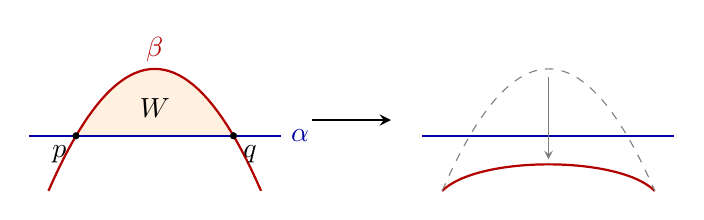
\begin{tikzpicture}[x=1cm,y=1cm,>=stealth]
	\begin{scope}
		\fill[orange!12] (-1,0) parabola bend (0,0.85) (1,0)--cycle;
		\draw[thick,blue!65!black] (-1.6,0)--(1.6,0) node[right] {\(\alpha\)};
		\draw[thick,red!70!black,domain=-1.35:1.35,samples=45] plot (\x,{0.85*(1-\x*\x)});
		\fill (-1,0) circle (1.3pt) node[below left] {\(p\)};
		\fill (1,0) circle (1.3pt) node[below right] {\(q\)};
		\node at (0,0.35) {\(W\)};
		\node[red!70!black] at (0,1.1) {\(\beta\)};
	\end{scope}
	\draw[->,thick] (2,0.2)--(3,0.2);
	\begin{scope}[xshift=5cm]
		\draw[thick,blue!65!black] (-1.6,0)--(1.6,0);
		\draw[thick,red!70!black] (-1.35,-0.7) .. controls (-0.9,-0.25) and (0.9,-0.25) .. (1.35,-0.7);
		\draw[dashed,gray,domain=-1.35:1.35,samples=45] plot (\x,{0.85*(1-\x*\x)});
		\draw[->,gray] (0,0.75)--(0,-0.3);
	\end{scope}
\end{tikzpicture}
